% * * * * * * * * * * * * * * * * * * * * * * * * * * * * * * * * * * * 
% *
% * Documentation programme cargol
% *
% * Germain Vallverdu
% * 26 02 2010
% * germain_vallverdu@yahoo.fr
% *
% * * * * * * * * * * * * * * * * * * * * * * * * * * * * * * * * * * *

\documentclass[11pt,a4paper,fleqn]{book}

% * * * * * * * * * * * * * * * * * * * * * * * * * * * * * * * * * * * 
% *
% * preambule
% *
% * * * * * * * * * * * * * * * * * * * * * * * * * * * * * * * * * * *

% * * * * * * * * * * * * * * * * * * * * * * * * * * * * * * * * * * * * * * *
% *
% * fichier entete de cargol.tex
% *
% * * * * * * * * * * * * * * * * * * * * * * * * * * * * * * * * * * * * * * *


% * * * * * * * * * * * * * * * * * * * * * * * * * * * * * * * * * * * * * * *
% * 
% * POLICE, ENCODAGE, LANGUE, FIGURES, COULEURS
% * 
% * * * * * * * * * * * * * * * * * * * * * * * * * * * * * * * * * * * * * * *

\usepackage[utf8]{inputenc}
\usepackage[T1]{fontenc}
\usepackage[francais]{babel}

\usepackage[svgnames]{xcolor}
\usepackage{graphicx,rotating,float,tikz}

\definecolor{turquoise}{rgb}{0 0.41 0.41}
\definecolor{rouge}{rgb}{0.79 0.0 0.1}
\definecolor{vert}{rgb}{0.15 0.4 0.1}
\definecolor{mauve}{rgb}{0.6 0.4 0.8}
\definecolor{violet}{rgb}{0.58 0. 0.41}
\definecolor{orange}{rgb}{0.8 0.4 0.2}
\definecolor{bleu}{rgb}{0.39 0.58 0.93}

\usepackage{url}

% * * * * * * * * * * * * * * * * * * * * * * * * * * * * * * * * * * * * * * *
% * 
% * MATHEMATIQUES
% * 
% * * * * * * * * * * * * * * * * * * * * * * * * * * * * * * * * * * * * * * *

\usepackage{amsmath, amsfonts, amssymb}

\setlength{\mathindent}{5ex} % position equation

% * * * * * * * * * * * * * * * * * * * * * * * * * * * * * * * * * * * * * * *
% * 
% * FORMAT DES PARAGRAPHE, ELARGISSEMENT DES TABLEAUX
% * 
% * * * * * * * * * * * * * * * * * * * * * * * * * * * * * * * * * * * * * * *

\setlength{\parskip}{1.5ex plus 0.5ex minus 0.5ex}	% espacement entre les paragraphes
\setlength{\parindent}{0em}        			% pas d'indentation
\usepackage{setspace}              			% pour gérer l'interligne

\usepackage{supertabular}
\usepackage{tabularx}

\renewcommand{\arraystretch}{1.4}  			% élargir les tableaux

% * * * * * * * * * * * * * * * * * * * * * * * * * * * * * * * * * * * * * * *
% * 
% * FOOTNOTE
% * 
% * * * * * * * * * * * * * * * * * * * * * * * * * * * * * * * * * * * * * * *

\renewcommand{\thefootnote}{\alph{footnote}}  
\newcounter{compteur}[page] 				% compteur asservis
\setcounter{compteur}{0}   
\newcommand{\myfoot}[1]{\hspace{0.5ex}\stepcounter{compteur}\footnote[\thecompteur]{#1}}
\renewcommand{\footnoterule}{\vspace{0.1cm}\rule{0.45\textwidth}{0.5pt}\vspace{0.5mm}}

% * * * * * * * * * * * * * * * * * * * * * * * * * * * * * * * * * * * * * * *
% * 
% * HYPERREF
% * 
% * * * * * * * * * * * * * * * * * * * * * * * * * * * * * * * * * * * * * * *

\usepackage{hyperref}

\hypersetup{% 
pdftex,%			Sets up hyperref for use with the pdftex program
colorlinks=true,% 		active les liens
citecolor=RoyalBlue,
linkcolor=RoyalBlue,
pdfborder={0 0 0},%		bordure des liens
pdfstartpage=1,%		page affichee a l'ouverture du pdf
pdfauthor={Germain Vallverdu},%
pdftitle={Code séquentiel de simulation de fluide simple},% 
pdfcreator={PDFLaTeX},%
pdfproducer={PDFLaTeX},%
}

% * * * * * * * * * * * * * * * * * * * * * * * * * * * * * * * * * * * * * * *
% * 
% * NOUVELLES COMMANDES
% * 
% * * * * * * * * * * * * * * * * * * * * * * * * * * * * * * * * * * * * * * *

\usepackage{xspace}
\newcommand{\eme}{$^{\text{ème}}$\xspace}%ième
\newcommand{\er}{$^{\text{er}}$\xspace}		%premier
\newcommand{\ere}{$^{\text{ère}}$\xspace}%première
\renewcommand{\degre}{$^{\circ}$\xspace}		% degre
\newcommand{\na}{\mathcal{N}_{a}\xspace}	% avogadro
\newcommand{\kt}{k_{\textrm{B}}T\xspace}	% kBT

\setlength\fboxsep{0pt}					% séparation text - contour
\setlength\fboxrule{1.5pt}				% eppaisseur du trait

% pour encadrer dans des equations
\newcommand{\encq}[2]{%
\tikz[baseline]{\node[rectangle,anchor=base,rounded corners,fill=#1]{#2};}}

% pour encadrer du texte dans un cadre rouge
\newcommand{\enc}[1]{%
\begin{center}
	\tikz{\node[rectangle,anchor=base,rounded corners,draw=rouge,thick,inner sep=2mm]{
		\parbox{0.9\textwidth}{ #1 }};}
\end{center}
}

\newcommand{\kw}[1]{ \textbf{\textsf{#1}} }

\newfloat{codesource}{htbp}{src}[chapter]
	% nom de mon nouvel environnement
	% htbp sont les options de placement de mon flottant
	% extension du fichier utilise pour construire la liste des flottants
	% niveau duquel dependra la numerotation des flottants
\floatname{codesource}{Code source} % titre du caption

% * * * * * * * * * * * * * * * * * * * * * * * * * * * * * * * * * * * * * * *
% * 
% * DEFINITION DU TITRE
% * 
% * * * * * * * * * * * * * * * * * * * * * * * * * * * * * * * * * * * * * * *

% * * * * * un titre simple aligné à droite dans une page
\makeatletter
\renewcommand{\maketitle}{
	\rule{\textwidth}{1pt}
	\vspace*{-8mm}
	\begin{flushright}
		\LARGE \bfseries \@title  \\
		\vspace*{5mm}
		\large \bfseries \@author \\
		\vspace*{4mm}
		\large \bfseries \@date \\
		\vspace*{-3mm}
	\end{flushright}
	\rule{\textwidth}{1pt} \\
}
\makeatother

% * * * * * * * * * * * * * * * * * * * * * * * * * * * * * * * * * * * 
% *
% * format de la page
% *
% * * * * * * * * * * * * * * * * * * * * * * * * * * * * * * * * * * *

\usepackage[nohead,top=2.5cm,bottom=2.5cm,left=2.5cm,right=2.5cm]{geometry}

\usepackage{fancyhdr}
\pagestyle{fancy}
\fancyhead{}                         % supprime toutes les entetes
\fancyfoot{}                         % supprime tous les pieds de page
\fancyfoot[LE,RO]{\footnotesize\thepage}          % le numero de page en bas a droite ou gauche
\fancyfoot[LO,RE]{\footnotesize\sffamily\itshape Cargol : G. Vallverdu}
\renewcommand{\headrulewidth}{0pt}
\renewcommand{\footrulewidth}{0pt}

% redefini le syle plain
\fancypagestyle{plain}{%
\fancyhf{}                           % clear all header and footer fields
\fancyfoot[RE,RO]{\thepage}
\renewcommand{\headrulewidth}{0pt}
\renewcommand{\footrulewidth}{0pt}}

% * * * * * * * * * * * * * * * * * * * * * * * * * * * * * * * * * * * 
% *
% * package listing
% *
% * * * * * * * * * * * * * * * * * * * * * * * * * * * * * * * * * * *

\usepackage{listings}
\lstset{% general command to set parameter(s)
language=C,                                     % langage
identifierstyle=,                               % rien
basicstyle=\footnotesize\sffamily,              % style du texte
stringstyle=\sffamily\color{green},             % styme typewriter pour string
keywordstyle=\color{DarkRed}\bfseries,        % style des mots clef
commentstyle=\color{RoyalBlue},                      % style commentaire
backgroundcolor=\color{black!3},                  % couleur arrière plan
}

% * * * * * * * * * * * * * * * * * * * * * * * * * * * * * * * * * * * 
% *
% * format titres et sections
% *
% * * * * * * * * * * * * * * * * * * * * * * * * * * * * * * * * * * *

\usepackage{titlesec}
% \titleformat{ command }[ shape ]{ format }{ label }{ sep }{ before }[ after ]
% \titlespacing*{ command }{ left }{ dessus }{ apres }

\titleformat{\chapter}[block]%
{\LARGE\bfseries\sffamily\filleft}%	% format
{\titlerule \\ \thechapter}%		% label
{2ex}%					% séparation label
{}%					% avant = (entre label et texte)
[\vspace{1ex} \titlerule]		% après
\titlespacing*{\chapter}{0cm}{0cm}{1cm}

\newcounter{gsec}[chapter]
\setcounter{gsec}{0}
\titleformat{\section}{\normalfont\Large\bfseries}{\stepcounter{gsec}\thegsec}{1em}{}
\titlespacing*{\section}{0ex}{3.5ex plus 1ex minus 0.2ex}{2.3ex plus .2ex}

\newcounter{gsubsec}[section]
\setcounter{gsubsec}{0}
\titleformat{\subsection}{\normalfont\large\bfseries}{\stepcounter{gsubsec}\thegsec.\thegsubsec}{1em}{}
\titlespacing*{\subsection}{0ex}{3.25ex plus 1ex minus 0.2ex}{1.5ex plus .2ex}

\titleformat{\subsubsection}[hang]{\bfseries}{}{0ex}{}
\titlespacing*{\subsubsection}{0ex}{2ex}{0ex}

%\usepackage{titletoc}
%\titlecontents{section}[10ex]{}{\sffamily\bfseries\Large\contentslabel{4ex}}{}
%{\sffamily\titlerule*[0.5pc]{.}\contentspage}[\vspace*{5ex}]

\usepackage{fncylab}
\labelformat{figure}{\sffamily \figurename~#1}
\labelformat{table}{\tablename~#1}
\labelformat{equation}{\sffamily équation~#1}
\labelformat{codesource}{\sffamily code source~#1}

% * * * * * * * * * * * * * * * * * * * * * * * * * * * * * * * * * * *

\graphicspath{{./images/}}

\title{Code de simulation séquentiel : cargol}
\author{Germain Vallverdu}
\date{\today}

% * * * * * * * * * * * * * * * * * * * * * * * * * * * * * * * * * * * 
% *
% * debut document
% *
% * * * * * * * * * * * * * * * * * * * * * * * * * * * * * * * * * * *

\begin{document}
\renewcommand{\labelitemi}{\hspace{3ex} $\bullet$} 
\renewcommand{\figurename}{figure}
\renewcommand{\tablename}{tableau}
\onehalfspacing

\thispagestyle{empty}
\maketitle

\begin{center}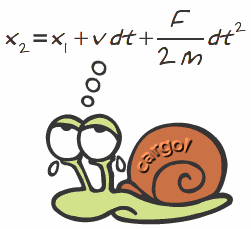
\includegraphics[scale=0.5]{logo}\end{center}

\vspace{2\baselineskip}

% * * * * * * * * * * * * * * * * * * * * * * * * * * * * * * * * * * * 
% *
% * resume
% *
% * * * * * * * * * * * * * * * * * * * * * * * * * * * * * * * * * * *

\begin{center}
\begin{minipage}{0.9\textwidth}
	\noindent\textbf{\large Présentation}\vspace*{0.7ex} \\
	Ce document présente un code de simulation séquentiel, écrit en langage C : cargol. 
	Ce code se limite à la simulation de fluides ou de solides composés de 
	particules identiques à un seul centre de force et dont l'interaction 
	est modélisée par un potentiel de paire. Beaucoup de code de simulation 
	moléculaire plus complet et bien plus efficace existe et ce code n'a pas
	d'intérêt dans la production de résultats.
	Le seul avantage de cargol est sa simplicité. Elle est due au fait que ses 
	possibilités sont limitées : en terme de systèmes, de potentiels et de 
	méthodes de calcul, mais aussi au fait que ce n'est pas un code parallèle.
	De ce fait l'ensemble du code contient seulement une vingtaine de fonctions.
	On peut alors facilement soit découvrir le contenu minimum d'un code de 
	simulation moléculaire de fluides simples, soit utiliser le code pour 
	développer et tester de nouvelles méthodes de simulations. \\
	
	Après avoir présenté les possibilités et l'utilisation du code, les notions 
	importantes de simulations qui sont présentes dans le code sont brièvement 
	rappelées.
\end{minipage}
\end{center}

% * * * * * * * * * * * * * * * * * * * * * * * * * * * * * * * * * * * 
% *
% * table des matières
% *
% * * * * * * * * * * * * * * * * * * * * * * * * * * * * * * * * * * *

\newpage
\thispagestyle{empty}

\setcounter{tocdepth}{1}
%\renewcommand{\contentsname}{Sommaire \\ \rule{\textwidth}{0.75pt}}
\renewcommand{\contentsname}{Sommaire}
\tableofcontents

\newpage
\thispagestyle{empty}

% * * * * * * * * * * * * * * * * * * * * * * * * * * * * * * * * * * * 
% *
% * Foncionnalités
% *
% * * * * * * * * * * * * * * * * * * * * * * * * * * * * * * * * * * *

\chapter{Fonctionnalités}

% * * * * * * * * * * * * * * * * * * * * * * * * * * * * * * * * * * * 
% *
% * Utilisation et fichiers d'entree sortie
% *
% * * * * * * * * * * * * * * * * * * * * * * * * * * * * * * * * * * *

\chapter{Utilisation et fichier d'entrée sortie}

\section{Description des mots clefs}

\subsection{Contrôle du calcul}

\begin{supertabular}{p{0.15\textwidth}p{0.12\textwidth}p{0.67\textwidth}}
	\kw{methode} & \multicolumn{2}{p{0.8\textwidth}}{Ce mot clef prend pour valeur une 
	chaîne de caractères. Il définit le type de calcul que l'on souhaite faire.} \\
	& \textit{brownien} & Mouvement brownien en deux dimensions. \\
	& \textit{NVE} & (defaut) Simulation de dynamique moléculaire dans l'ensemble 	
		microcanonique. \\
	& \textit{langevin} & Simulation de dynamique moléculaire dans l'ensemble canonique. Le
		système est couplé à un thermostat en utilisant une équation de Langevin
		(voir \ref{eq_langevin}) . \\
	& \textit{DPD} & Simulation de dynamique de particule dissipative dans l'ensemble 
		canonique (voir ?) . \\
	& \textit{DPDE} & Simulation de dynamique de particule dissipative dans l'ensemble 
		microcanonique (voir ?).  \\

	\kw{temp0 } & \multicolumn{2}{p{0.8\textwidth}}{Température de référence, en
	kelvin, utilisée pour calculer les vitesses initiales des particules. Pour 
	les simulation dans l'ensemble canonique il s'agit de la température
	du thermostat. Valeur par défaut 300~K.} \\

	\kw{nstep} & \multicolumn{2}{p{0.8\textwidth}}{Nombre de pas de simulation. 
	Defaut 1000} \\
	
	\kw{dt} & \multicolumn{2}{p{0.8\textwidth}}{Pas de temps en seconde. Defaut 1~fs.} \\

	\kw{xsi} & \multicolumn{2}{p{0.8\textwidth}}{Coefficient de friction utilisé dans
	les méthodes faisant intervenir une équation de Langevin (langevin, DPD, DPDE). xsi
	est donné en kg.s$^{-1}$. Défaut 1e-12 kg.s$^{-1}$.} \\

	\kw{vg\_initiale} & \textit{vgx,vgy,vgz} & Détermine la vitesse initiale
	de l'ensemble des particules, imposée selon l'axe $x$, $y$, $z$. Les vitesses
	selon les axes $x$, $y$ et $z$ doivent être données en m.s$^{-1}$ séparées 
	par des virgules et sans espaces. \\

	\kw{graine} & \multicolumn{2}{p{0.8\textwidth}}{C'est un nombre entier utilisée
	par le générateur de nombres aléatoires. Il détermine la série de nombres
	aléatoires. Défaut 64534.} \\
	
\end{supertabular}

\subsection{Contrôle des sorties}

\begin{supertabular}{p{0.15\textwidth}p{0.12\textwidth}p{0.67\textwidth}}

	\kw{nave} & \multicolumn{2}{p{0.8\textwidth}}{Tous les nave pas de temps, les 
	grandeurs moyennes sont recalculées et imprimées dans le fichier mdout.dat. Défaut
	5.} \\
	
	\kw{nout} & \multicolumn{2}{p{0.8\textwidth}}{Tous les nout pas de temps, les 
	grandeurs moyennes sont affichées à l'écran (sur la sortie standard). nout doit 
	être un multiple de nave. Défaut 1000.} \\
	
	\kw{ncrd} & \multicolumn{2}{p{0.8\textwidth}}{Tous les ncrd pas de temps, les 
	coordonnées cartésiennes des atomes sont écrites dans le fichier mdcrd.xyz. Si 
	ncrd > 0, le fichier mdcrd.xyz est écrasé à chaque nouvelle écriture. Si ncrd < 0,
	un fichier est sauvegardé tous les ncrd pas de temps sous le nom mdcrd\_XXX.xyz, où
	XXX est le numéro de l'itération. La valeur 0 annule la création des fichiers.
	Défaut 200.} \\
	
	\kw{nvel} & \multicolumn{2}{p{0.8\textwidth}}{Tous les nvel pas de temps, les 
	vitesses cartésiennes des atomes sont écrites dans le fichier mdvel.xyz. Si 
	nvel > 0, le fichier mdvel.xyz est écrasé à chaque nouvelle écriture. Si nvel < 0,
	un fichier est sauvegardé tous les nvel pas de temps sous le nom mdvel\_XXX.xyz, où
	XXX est le numéro de l'itération. La valeur 0 annule la création des fichiers.
	Défaut 0.} \\
	
	\kw{pas\_radial\_dist} & \multicolumn{2}{p{0.8\textwidth}}{Indique la
	largeur, en mètre, des intervalles utilisés pour construire la fonction 
	de distribution radiale : g(r). Défaut 0.1~\AA} \\

\end{supertabular}

\subsection{Distance de coupure et liste de voisins}

\begin{supertabular}{p{0.15\textwidth}p{0.1\textwidth}p{0.67\textwidth}}
	\kw{rcut} & \multicolumn{2}{p{0.8\textwidth}}{Distance de coupure, en mètre,
	des interactions de paires. Défaut 2.5$\sigma$.} \\

	\kw{rverlet} & \multicolumn{2}{p{0.8\textwidth}}{Distance de coupure, en mètre,
	utilisée pour construire les listes de voisins. Défaut 3.$\sigma$.} \\
	
	\kw{nbrevoisinmax} & \multicolumn{2}{p{0.8\textwidth}}{Nombre maximal de
	voisins enregistrés dans les listes de voisins. Pour des fortes densité le
	nombre de voisin peut être important. Si le nombre de voisin dépasse
	\textit{nbrevoisinmax} le calcul s'arrête. Défaut 100.} \\
\end{supertabular}

\subsection{Configuration initiale}

\begin{supertabular}{p{0.15\textwidth}p{0.1\textwidth}p{0.67\textwidth}}
	\kw{cristal} & \multicolumn{2}{p{0.8\textwidth}}{Détermine le type de
	réseau cristallin utilisé pour construire la configuration initiale.} \\
	& \textit{CFC} & maille cubique face centrée, 4 atomes par maille. \\
	& \textit{centre} & maille cubique centrée, 2 atomes par maille. \\
	& \textit{simple} & (défaut) maille cubique simple, 1 atomes par maille. \\

	\kw{a0} & \multicolumn{2}{p{0.8\textwidth}}{Longueur des arrêtes de la
	maille en mètres. Défaut 5.\AA} \\
	
	\kw{dimension} & $N_x,N_y,N_z$ & Indique sous la forme d'un triplet de nombre
	entier, le nombre de fois que la maille doit être rajoutée dans chaque direction
	$x$, $y$ et $z$ pour construire la configuration initiale et la boîte de simulation.
	Les trois nombres entier doivent être donnés séparés par des virgules et sans espaces.
	Défaut 10,10,10. \\
	
	\kw{restart} & \multicolumn{2}{p{0.8\textwidth}}{Indique si la configuration
	initiale doit être construire ou lue sur un fichier.} \\
	& \textit{non} & (défaut) la configuration initiale est construite. \\
	& \textit{fichier} & La configuration initiale est lue sur le fichier 
	\textit{fichier}. \\
	
\end{supertabular}

\subsection{paramètres du potentiel et des atomes}

Les paramètres par défaut correspondent à ceux de l'argon.

\begin{supertabular}{p{0.15\textwidth}p{0.1\textwidth}p{0.67\textwidth}}
	\kw{aname} & \multicolumn{2}{p{0.8\textwidth}}{Indique le nom de l'atome.
	Défaut Ar.} \\

	\kw{masse} & \multicolumn{2}{p{0.8\textwidth}}{Donne la masse molaire de 
	l'atome en kg.mol$^{-1}$. Défaut 39.95e-3 kg.mol$^{-1}$.} \\

	\kw{LJsigma} & \multicolumn{2}{p{0.8\textwidth}}{Paramètre $\sigma$ du
	potentiel Lenard Jones en mètre. Défaut 3.405e-10 m.} \\
	
	\kw{LJeps} & \multicolumn{2}{p{0.8\textwidth}}{Paramètre $\epsilon$ du
	potentiel Lenard Jones en joule. Défaut 1.6567944e-21 J.} \\
\end{supertabular}

\section{Fichier d'entrée}

Le fichier d'entrée du programme est un fichier texte contenant un
mot clef et la valeur qu'on lui attribue par ligne. L'ordre des mots
clefs et le nom du fichier d'entrée n'ont pas d'importance. Les 
lignes commençant par les caractères \# ou * sont ignorées et peuvent servir
de commentaires. 

Il n'est pas nécessaire d'indiquer tous les mots clefs dans le fichier
d'entrée. Si certains mots clefs sont absent le programme leur attribu
une valeur par défaut. Le \ref{code_input} présente
un fichier d'entrée avec tous les mots clefs et la valeur qu'ils
prennent s'ils ne sont pas spécifiés.

\begin{codesource}[htbp]
\begin{lstlisting}[language=bash]
# ----------------------------------------------------------
#
#   fichier input complet avec les valeurs par defaut
#
# ----------------------------------------------------------
#
# controle du calcul
methode		NVE
temp0	 	300.e0
nstep		1000
dt		0.001e-12
xsi 		1e-12.
vg_initiale	0.,0.,0.
graine		64534
# controle des sorties
nave		5
nout		1000
ncrd		200
nvel		0
pas_radial_dist	0.1e-10
# cut off et voisins
rcut		8.5125e-10
rverlet		10.6125e-10
nbrevoisinmax	100
# geometrie initiale 
cristal		simple
a0			5.0e-10
dimension	10,10,10
restart		non
# parametres du potentiel et des atomes
aname		Ar
masse		39.95e-3
LJsigma		3.405e-10
LJeps		1.6567944e-21
\end{lstlisting}
\caption{Exemple d'un fichier d'entrée du programme. Tous les mots
clefs sont présents avec leur valeur par défaut.}
\label{code_input}
\end{codesource}

% * * * * * * * * * * * * * * * * * * * * * * * * * * * * * * * * * * * 
% *
% * Description du code
% *
% * * * * * * * * * * * * * * * * * * * * * * * * * * * * * * * * * * *

\chapter{Description du code}

Les fonctions l'organiation, présentation des sources

% * * * * * * * * * * * * * * * * * * * * * * * * * * * * * * * * * * * 
% *
% * Notions de simulation utilisées dans le code
% *
% * * * * * * * * * * * * * * * * * * * * * * * * * * * * * * * * * * *

\chapter{Notions de simulations utilisées dans le code}

\section{Mouvement brownien simple}

Pur mouvement brownien, à chaque pas le mouvement est aléatoire. Les pas aléatoires
sont gaussiens et non corrélés.
%
\begin{equation*}
	d x \, = \, \sigma d W_t
\end{equation*}
%
Le terme $\sigma d W_t$ est un Brownien. Algorithme :
%
\begin{equation*}
	x^{n+1} \, = \, x^n \, + \, \mathring{x}
\end{equation*}
%
où $\mathring{x}$ est un déplacement aléatoire gaussien de moyenne nulle et 
de largeur $\sigma \sqrt{\Delta t}$ :
%
\begin{equation}\label{eq_dx_rand}
	\rho(\mathring{x}) \, \propto \, exp\left( -\frac{x^2}{2 \sigma^2 \Delta t} \right)
		\, = \, \mathcal{N}(0,\sigma^2 \Delta t)
\end{equation}
%
Il en découle que la largeur de la distribution des valeurs de $x$ tend vers
$\sigma \sqrt(\Delta t)$. 

% * * * * * * * * * * * * * * * * * * * * * * * * * * * * * * * * * * *

\section{Simulation dans l'ensemble micro-canonique : NVE}

% * * * * * * * * * * * * * * * * * * * * * * * * * * * * * * * * * * *

\section{Simulation dans l'ensemble canonique : NVT}

Equation de langevin, toutes les coordonnées échanges de l'énergie avec
l'environnement sous forme d'une friction et d'un terme aléatoire :
%
\begin{eqnarray}
	m dv & = & F(x) dt - \gamma v dt + \sigma dWt \label{eq_langevin}
\end{eqnarray}
%
\begin{itemize}
	\item premier 1/2 pas de vitesse

	\begin{eqnarray*}
		v^{n+1/2} & = & v^n + \frac{\Delta t}{2m} \, F(x^n) \\
	\end{eqnarray*}

	\item 1 pas complet pour les positions

	\begin{eqnarray*}
		x^{n+1} & = & x^n + \Delta t v^{n+1/2} \\
	\end{eqnarray*}

	\item A ce stade on a fait exactement un pas NVE. \\

	\item Calcul des forces pour $x^{n+1}$ \\

	\item deuxième 1/2 pas vitesse avec prise en compte de la friction
	et du terme aléatoire.

	\begin{eqnarray*}
		\tilde v^{n+1} & = &  v^{n+1/2} + \frac{\Delta t}{2m} \, F(x^{n+1}) \\
		\alpha & = & exp\left(-\dfrac{\gamma t}{m}\right) \\
		v^{n+1} & = & \alpha \tilde v^{n+1} + 
			\sqrt{\dfrac{k_B\,T}{m}(1-\alpha^2)} \mathcal{N}(0,1) \\
	\end{eqnarray*}
\end{itemize}

\textbf{Remarques :}
\begin{itemize}
	\item La friction est exprimée en $kg.s^{-1}$, unités habituelles. Elle
	prend des valeurs de l'ordre de 1e-10 à 1e-14 $kg.s^{-1}$. \\

	\item on vérifie que pour $\gamma$=0 on retrouve NVE (voir figure). \\

	\item $\alpha$ pondère Langevin par rapport à NVE. Pour $\alpha$=1
	on a un langevin (voir brownien tout court ?) et pour $\alpha$=0 on
	a un NVE. \\

	\item avantages par rapport à l'autre algorithme ?
\end{itemize}

% * * * * * * * * * * * * * * * * * * * * * * * * * * * * * * * * * * *

\section{Calcul des forces et de l'énergie}

En simulation de dynamique moléculaire le calcul des forces est nécessaire
pour l'intégration des équations du mouvements des particules. La modélisation
des forces est une étape importante car elle détermine le sens physique que
l'on donne à la simulation. Le calcul des forces est très important également
car c'est la tache qui nécessite le plus de temps de calcul lors d'une simulation. 
Les algorithmes permettant de réduire le temps de calcul des forces seront
décrit au paragraphe suivant. Ce paragraphe abordera l'expression des
potentiels les plus courant et des forces utilisés qui en dérivent.

\subsection{Le potentiel Lenard Jones}

\subsubsection{Expression}

L'expression d'un potentiel Lenard Jones est donnée \ref{eq_potLJ}.
C'est un potentiel de paire qui dépend de deux paramètres $\epsilon$ et 
$\sigma$ qui définissent respectivement la profondeur du potentiel et
la distance d'équilibre. 
%
\begin{equation}\label{eq_potLJ}
	E_{LJ}(r) \, = \, 4 \epsilon \, \left[ \left(\frac{\sigma}{r}\right)^{12} 
			- \left(\frac{\sigma}{r}\right)^6 \right]
\end{equation}
%
Un potentiel Lenard Jones vaut 0 pour une distance égale à $\sigma$ et il 
vaut $-\epsilon$, son minimum, pour une distance égale à $R_o = 2^{1/6}\sigma$ 
($R_o\simeq1.12\sigma$). La \ref{fig_potLJ} représente le potentiel Lenard Jones 
avec les paramètres de l'argon.

\begin{figure}[htb]
	\begin{center}
		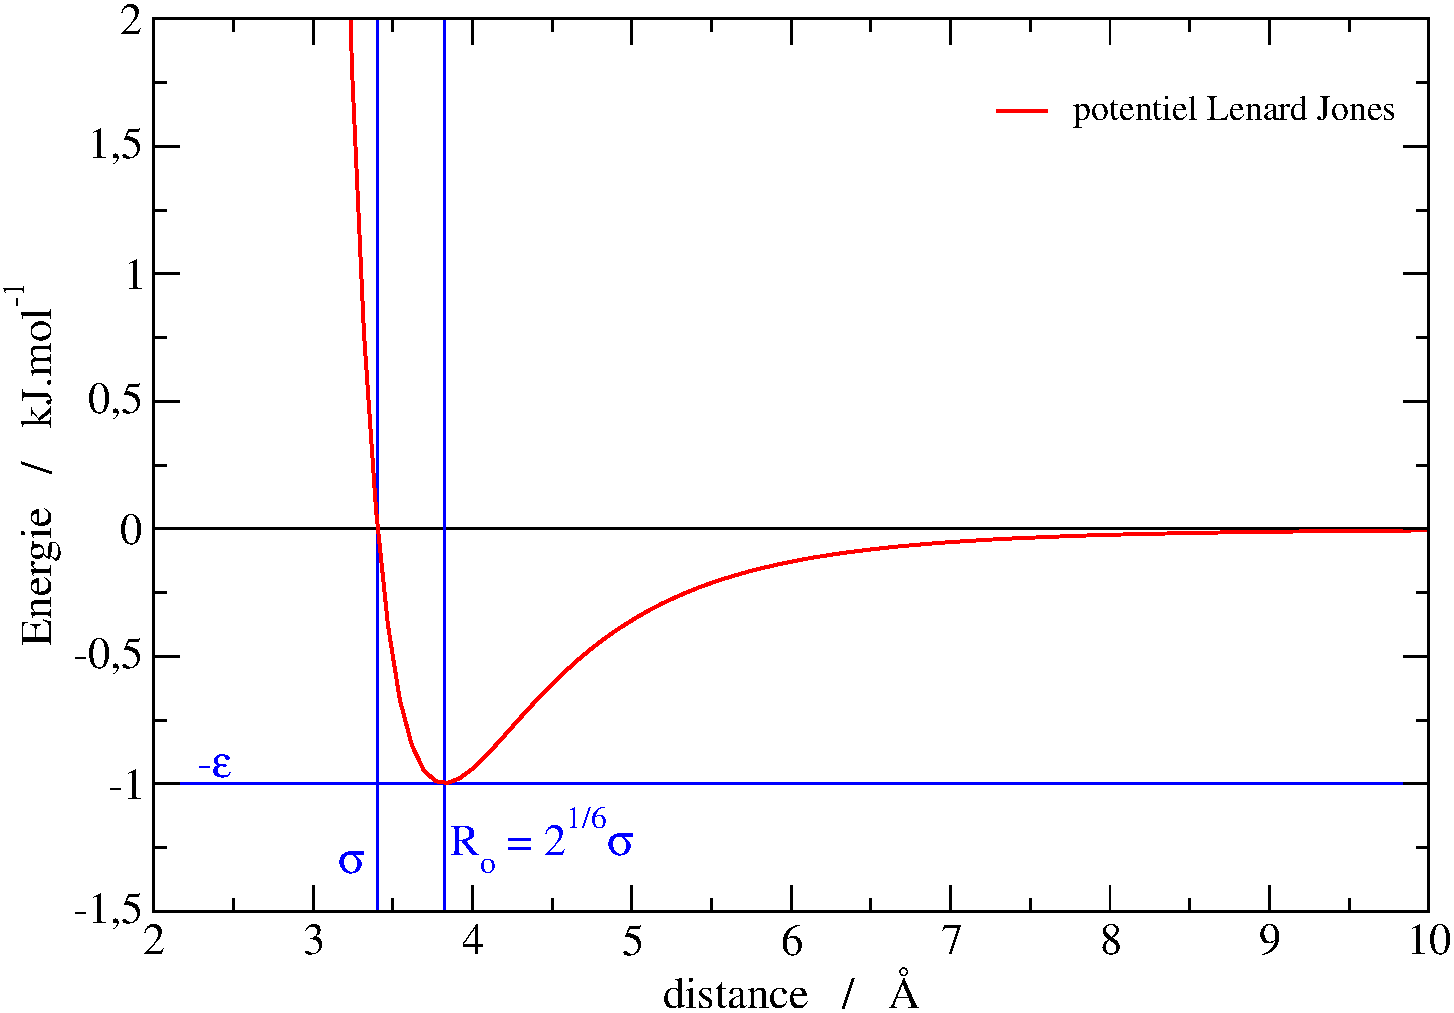
\includegraphics[width=0.6\textwidth]{potLJ}
	\end{center}
	\caption{Potentiel de type Lernard Jones et quelques points particulier.}
	\label{fig_potLJ}
\end{figure}

Parfois on préfère utiliser le paramètre $R_o$, la position du minimum, à la
place de $\sigma$. Dans ce cas l'expression du potentiel devient :
%
\begin{equation}
	E_{LJ}(r) \, = \, \epsilon \, \left[ \left(\frac{R_o}{r}\right)^{12} 
		- 2 \left(\frac{R_o}{r}\right)^6 \right]
\end{equation}
%
Affin de réduire le temps de calcul, le potentiel
Lenard Jones se calcule de la façon suivante :
%
\begin{equation*}
	E_{LJ}(r) \, = \, 4 \epsilon \, \left(\frac{\sigma}{r}\right)^6 
		\left[\left(\frac{\sigma}{r}\right)^6 - 1 \right]
\end{equation*}
%
Cette expression permet de se limiter à un seul calcul de la puissance 6 
du terme $\sigma/r$, le terme à la puissance 12 étant obtenu par multiplication.
La puissance 12 dans le potentiel a d'ailleurs été choisie
pour pouvoir écrire le potentiel sous cette forme\myfoot{Le terme en puissance 6
a par contre un sens physique, il correspond à une interaction de type
dipôle-dipôle.}.

\subsubsection{Calcul des forces}

Pour calculer la trajectoires des atomes au cours d'une dynamique on utilise 
les coordonnées cartésiennes dont les dérivées sont plus faciles à calculer.
Pour calculer les forces exercées sur chaque atome, on va donc également utiliser
les coordonnées cartésiennes. Dans le cas d'un potentiel de paire ce calcul est
simple car le potentiel ne dépend que de la distance entre deux particules qui
a une expression très simple en fonction des coordonnées cartésiennes. Les forces
sont données par le gradient du potentiel :
%
\begin{eqnarray}
	\overrightarrow{F_i} & = & - \overrightarrow{\nabla_i} \, E_{LJ}
\end{eqnarray}
%
Pour obtenir les forces on procède en deux étapes : on commence par
calculer la dérivée du potentiel par rapport à la distance entre les
deux particules, puis on calcule la dérivée de cette distance par rapport
aux coordonnées cartésiennes :
%
\begin{eqnarray*}
	F_{x,j\rightarrow i} & = & -\frac{d E_{LJ}}{d r_{ij}}\,\frac{\partial r_{ij}}{\partial x_i} \\
	F_{x,j\rightarrow i} & = & -\mathcal{D}_r \, \mathcal{D}_x
\end{eqnarray*}
%
où $F_{x,j\rightarrow i}$ est la force exercée par l'atome $j$ sur l'atome $i$ projetée
sur l'axe $x$, $r_{ij}$ est la distance entre les atomes $i$ et $j$ et $x_i$ est
la coordonnée sur l'axe $x$ de l'atome $i$. On remarquera que $\mathcal{D}_r$ est
indépendant de l'axe que l'on considère ($x$, $y$ ou $z$) et que $\mathcal{D}_x$
nécessairement en dépend. En revanche $\mathcal{D}_x$ ne dépend pas du potentiel. 
On obtient alors les expressions suivantes :
%
\begin{eqnarray}
	\mathcal{D}_r & = &  4 \epsilon \, \left(\frac{\sigma}{r_{ij}}\right)^6
		\left[ 6 - 12 \left(\frac{\sigma}{r_{ij}}\right)^6 
		\right]\frac{1}{r_{ij}} \label{eq_force_df}\\
	\mathcal{D}_x & = & - \frac{x_j-x_i}{r_{ij}} \label{eq_force_axe}
\end{eqnarray}
%
En pratique $\mathcal{D}_r$ est valable pour les trois
axes et ne sera donc calculé qu'une seule fois.
Comme pour le calcul de l'énergie, l'\ref{eq_force_df}
permet de limiter le nombre d'opérations à effectuer pour calculer les forces. 
De plus on pourra utiliser, pour ce calcul, ceux qui ont été
fait pour obtenir l'énergie (notamment le calcul de $\sigma/r$ à la puissance
6). Le calcul des forces et de l'énergie potentielle doit donc se faire 
si possible au même endroit pour limiter le temps de calcul. 
On a donc l'expression suivantes des forces sur l'axe $x$ :
%
\begin{eqnarray*}
	F_{x,j\rightarrow i} & = & 4 \epsilon \, \left(\frac{\sigma}{r_{ij}}\right)^6
		\left[ 6 - 12 \left(\frac{\sigma}{r_{ij}}\right)^6 
		\right]\left(\frac{1}{r_{ij}}\right)^2 
		\left(x_j-x_i\right)\\
\end{eqnarray*}
%
On a une expression similaire sur $y$ et $z$.

\subsection{Le potentiel exponnentielle-6}

\subsubsection{Expression}

Le potentiel exponnentielle-6, a une expression identique au potentiel Lenard
Jones pour la partie attractive du potentiel avec un terme en $1/r^6$. La partie
répulsive est représentée par une exponnentielle décroissante. Ce potentiel 
utilise 3 paramètres.
%
\begin{equation} \label{eq_pot_exp-6}
	E_{exp-6}(r) = A e^{-Br} - \frac{C}{r^6}
\end{equation}
%
L'évaluation de la fonction exponnentielle fait que ce potentiel est légèrement
plus couteux en temps de calcul qu'un potentiel Lenard Jones. La fonction
exponnentielle permet cependant une meilleure description des interactions
répulsives ce qui fait que ce potentiel est meilleur que le potentiel
Lenard Jones à courte distance. De ce fait, à très haute pression il
est préférable d'utiliser un potentiel avec une partie répulsive
modélisée par une exponnentielle.

\subsubsection{Calcul des forces}

Comme pour le potentiel Lenard Jones, on procède en deux étapes pour 
calculer les forces en séparant le calcul de $\mathcal{D}_r$ et de
$\mathcal{D}_x$ :
%
\begin{eqnarray*}
	F_{x,j\rightarrow i} & = & -\frac{d E_{exp-6}}{d r_{ij}}\,\frac{\partial r_{ij}}{\partial x_i} \\
	F_{x,j\rightarrow i} & = & -\mathcal{D}_r \, \mathcal{D}_x \nonumber
\end{eqnarray*}
%
On obtient l'expression suivante pour $\mathcal{D}_r$ :
%
\begin{eqnarray}
	\mathcal{D}_r & = & -AB e^{-Br} + \frac{6C}{r^7}
\end{eqnarray}
%
En pratique il est important de sauvegarder séparément chacun des termes
du potentiels pour pouvoir les utiliser à nouveau dans le calcul
des forces. Sur l'axe $x$, l'expression finale des forces est : 
%
\begin{eqnarray*}
	F_{x,j\rightarrow i} & = & \frac{x_j-x_i}{r}\left(\frac{6C}{r^7}-AB e^{-Br} \right)\\
\end{eqnarray*}
%
On a une expression similaire sur $y$ et $z$.

\subsection{Le potentiel de Morse}

\subsubsection{Expression}

Le potentiel de Morse a été initialement utilisé pour représenter l'énergie
d'une molécule diatomique en fonction de l'élongation de sa liaison. Il trouve
un grand nombre d'application en spectroscopie. Cependant il a une forme
assez proche des potentiels précédents et est aussi utilisé en simulation
classique. Le potentiel de Morse est simplement constitué d'une exponnentielle
décroissante et contient 3 paramètres.
%
\begin{equation}\label{eq_pot_morse}
	E_{Morse}(r) = \mathcal{D}_e\left[ 1 - e^{-\alpha(r-R_o) }\right]^2
\end{equation}
%
$\mathcal{D}_e$ correspond au paramètre $\epsilon$ du potentiel Lenard Jones
et représente la profondeur du puits, $R_o$ est la distance d'équilibre
et correspond au minimum du potentiel, $\alpha$ correspond à la raideur
du puits. 

\subsubsection{Calcul des forces}

Comme pour les potentiels précédents, on procède en deux étapes pour 
calculer les forces en séparant le calcul de $\mathcal{D}_r$ et de
$\mathcal{D}_x$ :
%
\begin{eqnarray*}
	F_{x,j\rightarrow i} & = & -\frac{d E_{Morse}}{d r_{ij}}\,\frac{\partial r_{ij}}{\partial x_i} \\
	F_{x,j\rightarrow i} & = & -\mathcal{D}_r \, \mathcal{D}_x \nonumber
\end{eqnarray*}
%
On obtient l'expression suivante pour $\mathcal{D}_r$ :
%
\begin{eqnarray}
	\mathcal{D}_r & = & 2 \mathcal{D}_e \, \alpha \, e^{-\alpha(r-R_o)}\left( 1 - e^{-\alpha(r-R_o) }\right)
\end{eqnarray}
%
Sur l'axe $x$, l'expression finale des forces est : 
%
\begin{eqnarray*}
	F_{x,j\rightarrow i} & = & 2\mathcal{D}_e \, \alpha \, e^{-\alpha(r-R_o)}
		\left( 1 - e^{-\alpha(r-R_o) }\right)\frac{x_j-x_i}{r}\\
\end{eqnarray*}
%
On a une expression similaire sur $y$ et $z$.

% * * * * * * * * * * * * * * * * * * * * * * * * * * * * * * * * * * * * * * * * * * * *

\section{Algorithme et symétrie du calcul des forces}

\subsection{Calucl des forces symétrique}

Etant donnée que l'on considère des interactions entre paires de particules,
le principe des actions réciproques impose :
%
\begin{eqnarray*}
	F_{x,j\rightarrow i} & = & - F_{x,i->j}
\end{eqnarray*}
%
Lors du calcul des forces on ne calculera qu'un seul de ces termes
en ajoutant systématiquement à la force subie par l'atome $j$, l'opposé
de la force subie par l'atome $i$. Le \ref{code_force_simple} présente
un algorithme simple de calcul des forces dues à un potentiel de type 
Lenard Jones.

\begin{codesource}[htbp]
\begin{lstlisting}

 /* les coordonnees x, y, z des atomes sont des variables externes
  * nat est le nombre d'atome total
  * les forces frcx, frcy et frcz d'un atome sont des variables externes
  * LJsigma6 est le parametre sigma a la puissance 6
  * LJ4eps est le parametre epsilon multiplie par 4 */

 void force_ene( void ) {

	int 	iat, jat ;
	double	xij, yij, zij ;
	double	fx, fy, fz, df ;
	double	dist2, dist_inv2, dist_inv6 ;
	double	ene, coef ;

	for ( iat = 0 ; iat < nat-1 ; iat++ ) {

		for ( jat = iat+1 ; jat < nat ; jat++ ) {

			// vecteur iat -> jat
			xij = x[jat] - x[iat] ;
			yij = y[jat] - y[iat] ;
			zij = z[jat] - z[iat] ;

			// distance iat - jat au carre
			dist2 = xij * xij + yij * yij + zij * zij ;
			dist_inv2 = 1. / dist2 ;
			dist_inv6 = dist_inv2 * dist_inv2 * dist_inv2 ;

			// energie
			coef = LJ4eps * dist_inv6 * LJsigma6 ;
			ene = coef * ( LJsigma6 * dist_inv6 - 1.0 ) ;
				
			// derivee par rapport a dist puis aux coordonnees xyz
			df = coef * ( 6. - 12. * LJsigma6 * dist_inv6 ) ;
			df = df * dist_inv2 ;

			fx = df * xij ;
			fy = df * yij ;
			fz = df * zij ;

			// mise a jour des forces
			frcx[iat] += fx ;
			frcy[iat] += fy ;
			frcz[iat] += fz ;

			frcx[jat] -= fx ;
			frcy[jat] -= fy ;
			frcz[jat] -= fz ;

			// mise a jour de l'energie potentielle
			eptot += ene ;

		}
	}
 }
\end{lstlisting}
	\caption{Calcul des forces dues à un potentiel Lenard Jones}
	\label{code_force_simple}
\end{codesource}


\subsection{Optimisation du calcul des forces}

Liste de voisins

\section{Calcul de grandeurs moyennes ou thermodynamique}

\subsection{Calcul de la température}

Dans une simulation de dynamique moléculaire la température est facilement
calculée étant donné que à tout instant on connait les vitesses de toutes 
les particules. On peut donc calculer la température à partir de l'énergie
cinétique totale du système :
%
\begin{eqnarray}
	E_{cinetique} & =  & \frac{3}{2}N k_B T \\
	T & = & \frac{2 \, E_{cinetique}}{3 N k_B}
\end{eqnarray}

Cette température est aussi appelée température cinétique du fait qu'elle
est calculée à partir des vitesses des particules.

\subsection{Calcul de la pression}

La pression qui s'exerce sur le système est calculée par la méthode du 
viriel (Allen et Tildesley page 47). Cette méthode s'applique dans le cas
où les interactions sont décrites par un potentiel de paires additif. Elle
est donc bien adaptée au cas présent qui utilise un potentiel Lenard Jones.
En dimension 3, la pression est donnée par :
%
\begin{eqnarray}\label{eq_viriel1}
	P\,V & = & N \, k_B \, T + \frac{1}{3}\sum_i \vec{f}_i \, \cdot \, \vec{r}_i
\end{eqnarray}
%
Le premier terme de cette équation correspond à la pression qu'aurait le
système s'il s'agissait d'un gaz parfait. Le viriel correspond au second 
terme de cette expression et fait intervenir les interactions entre
les particules.

Pour calculer la pression au cours d'une simulation il est préférable
d'utiliser une expression du viriel faisant intervenir les positions relatives des
particules. Du fait que les interactions que l'on considère sont des
interactions de paires additives, l'\ref{eq_viriel1} peut
s'écrire également :
%
\begin{eqnarray}\label{eq_viriel2}
	P & = & \frac{N \, k_B \, T}{V} + \frac{1}{3V}\sum_i \sum_{j<i} 
		\vec{f}_{ij} \, \cdot \, \vec{r}_{ij}
\end{eqnarray}
%
Le premier avantage de cette équation est que le viriel est
indépendant de l'origine des coordonnées du système. Deuxièmement
son calcul s'insère facilement au moment du calcul des forces.

\end{document}
